\subsection{Higgs boson at CMS}
\label{section_sm_vb_results}

The Higgs may be produced at LHC proton-proton collisions by the following process, called \mbox{\textbf{Production Modes}}. \textit{state-of-art} SM cross section predictions were computed by the "LHC Higgs Cross Section Working Group"\cite{deFlorian:2016spz} and are presented as a function oftheHiggs mass is presented at Figure~\ref{higgs_prod_modes} and examples of leading order Feynmann diagrams of them are presented at Figure~\ref{fig_diagrams_production_modes}, for the highest cross section production modes.

The \textbf{Gluon Fusion - ggF} - is the result of a gluon-gluon interaction which is mediated by a heavy quark loop. Each quark contributing is suppressed by $1/m_{q}^{2}$. It is by far the one with highest cross section. Its final state is composed only by a Higgs boson, which makes it harder to identify, since there are no other auxiliary final state particle to tag it. In this decay, QCD radiactive corrections are very important and have been in included in the results of Figure~\ref{higgs_prod_modes} up to N3LO (next-to-next-to-next-to-leading order, while electroweak corrections are computed up to NNLO. The \textbf{Associated Vector Boson Production - VH} - a SM vector boson (Z or W) irradiate a Higgs. Due to its clear electroweak signature (a final state with a Higgs and a vector boson), this production mode enhances the signal, when the Higgs decay has a large contribution from QCD background, e.g. $H \rightarrow b\bar{b}$. This process is also called Higgs-Strahlung.

The third process is the \textbf{Vector Boson Fusion - VBFH} - in which the two quarks from the initial state scatter by the emission a pair of vector bosons (ZZ or $W{\pm}W{\mp}$). Those would interact (fuse) and produce a Higgs in the final, associated with two back-to-back jets, from the initial state quarks. The \textbf{Associated $t\bar{t}$ Production - ttH} - and \textbf{Associated $b\bar{b}$Production - bbH} are very similar process (especially in the scale of $\sqrt{s} = 13$ TeV, where their cross sections almost match), where the coupling of the heavy quark to the Higgs boson, contrary to what happens in the ggF production, it is not with a virtual state of then. 

The \textbf{Associated Single Top Production - tH} - is the production mode with the smallest cross section, due to its destructive interference with other process. Without loss of generality, it is not considered in this study.


\begin{figure}[htbp]
  \centering
  \begin{subfigure}[htbp]{0.48\textwidth}
    \centering
    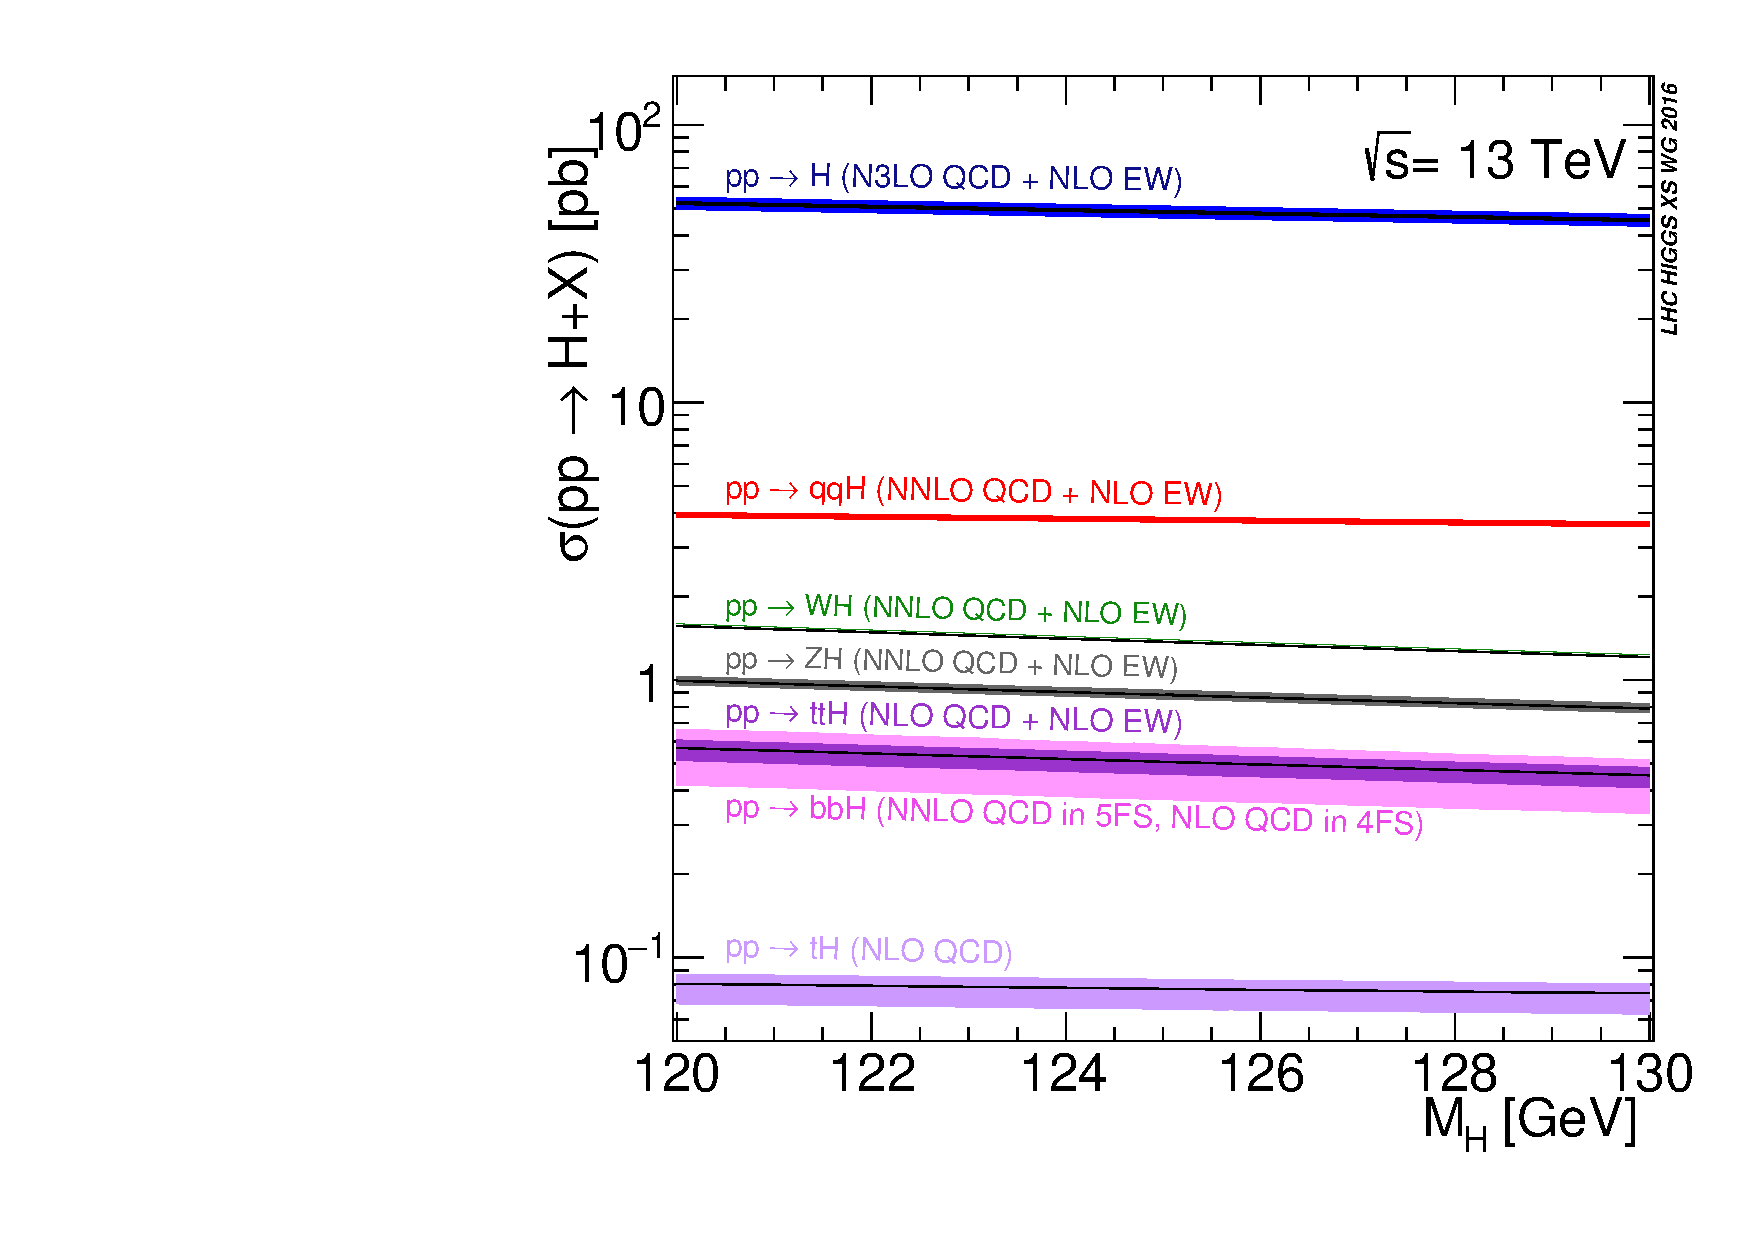
\includegraphics[width=\textwidth]{figures_and_tables/theory/higgs_prod_modes.pdf}
    \caption{}
    \label{higgs_prod_modes}
  \end{subfigure}
  \hfill
  \begin{subfigure}[htbp]{0.48\textwidth}
    \centering
    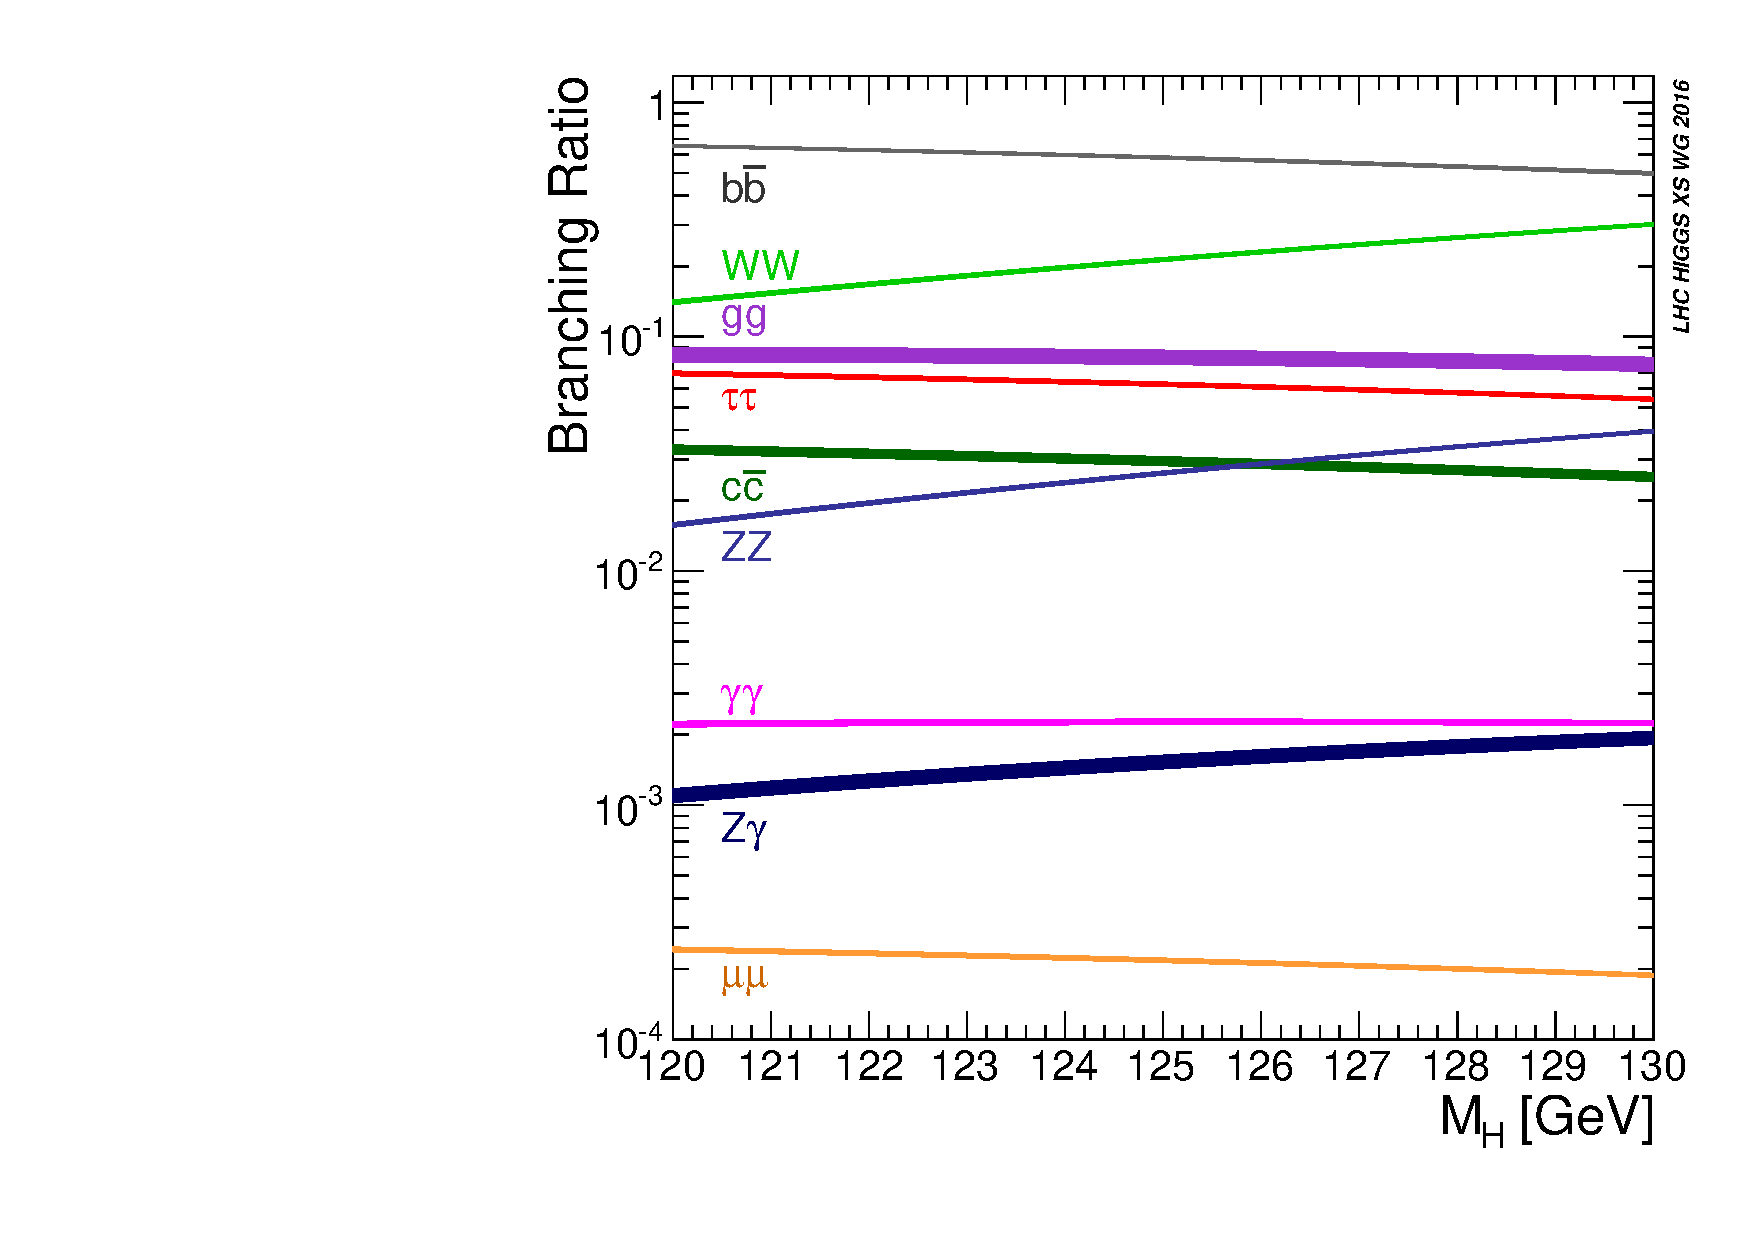
\includegraphics[width=\textwidth]{figures_and_tables/theory/higgs_decays.pdf}
    \caption{}
    \label{higgs_decays}
  \end{subfigure}
  \caption{(a) Standard Model Higgs boson production cross sections at $\sqrt{s}=13$ TeV as a function of Higgs boson mass. The tH production cross section accounts for $t$-channel and $s$-channel only (no $tWH$ production). The VBF process is indicated here as $qqH$. The theoretical uncertainties are indicated as shaded bands around the lines. Source:~\cite{deFlorian:2016spz}. (b) Standard Model Higgs boson decay branching ratios for different decay channels. The theoretical uncertainties are indicated as shaded bands around the lines. Source:~\cite{deFlorian:2016spz}.}
\end{figure}

% production modes
\begin{figure}[htbp]
  \centering
  \begin{subfigure}[htbp]{0.48\textwidth}
    \centering
    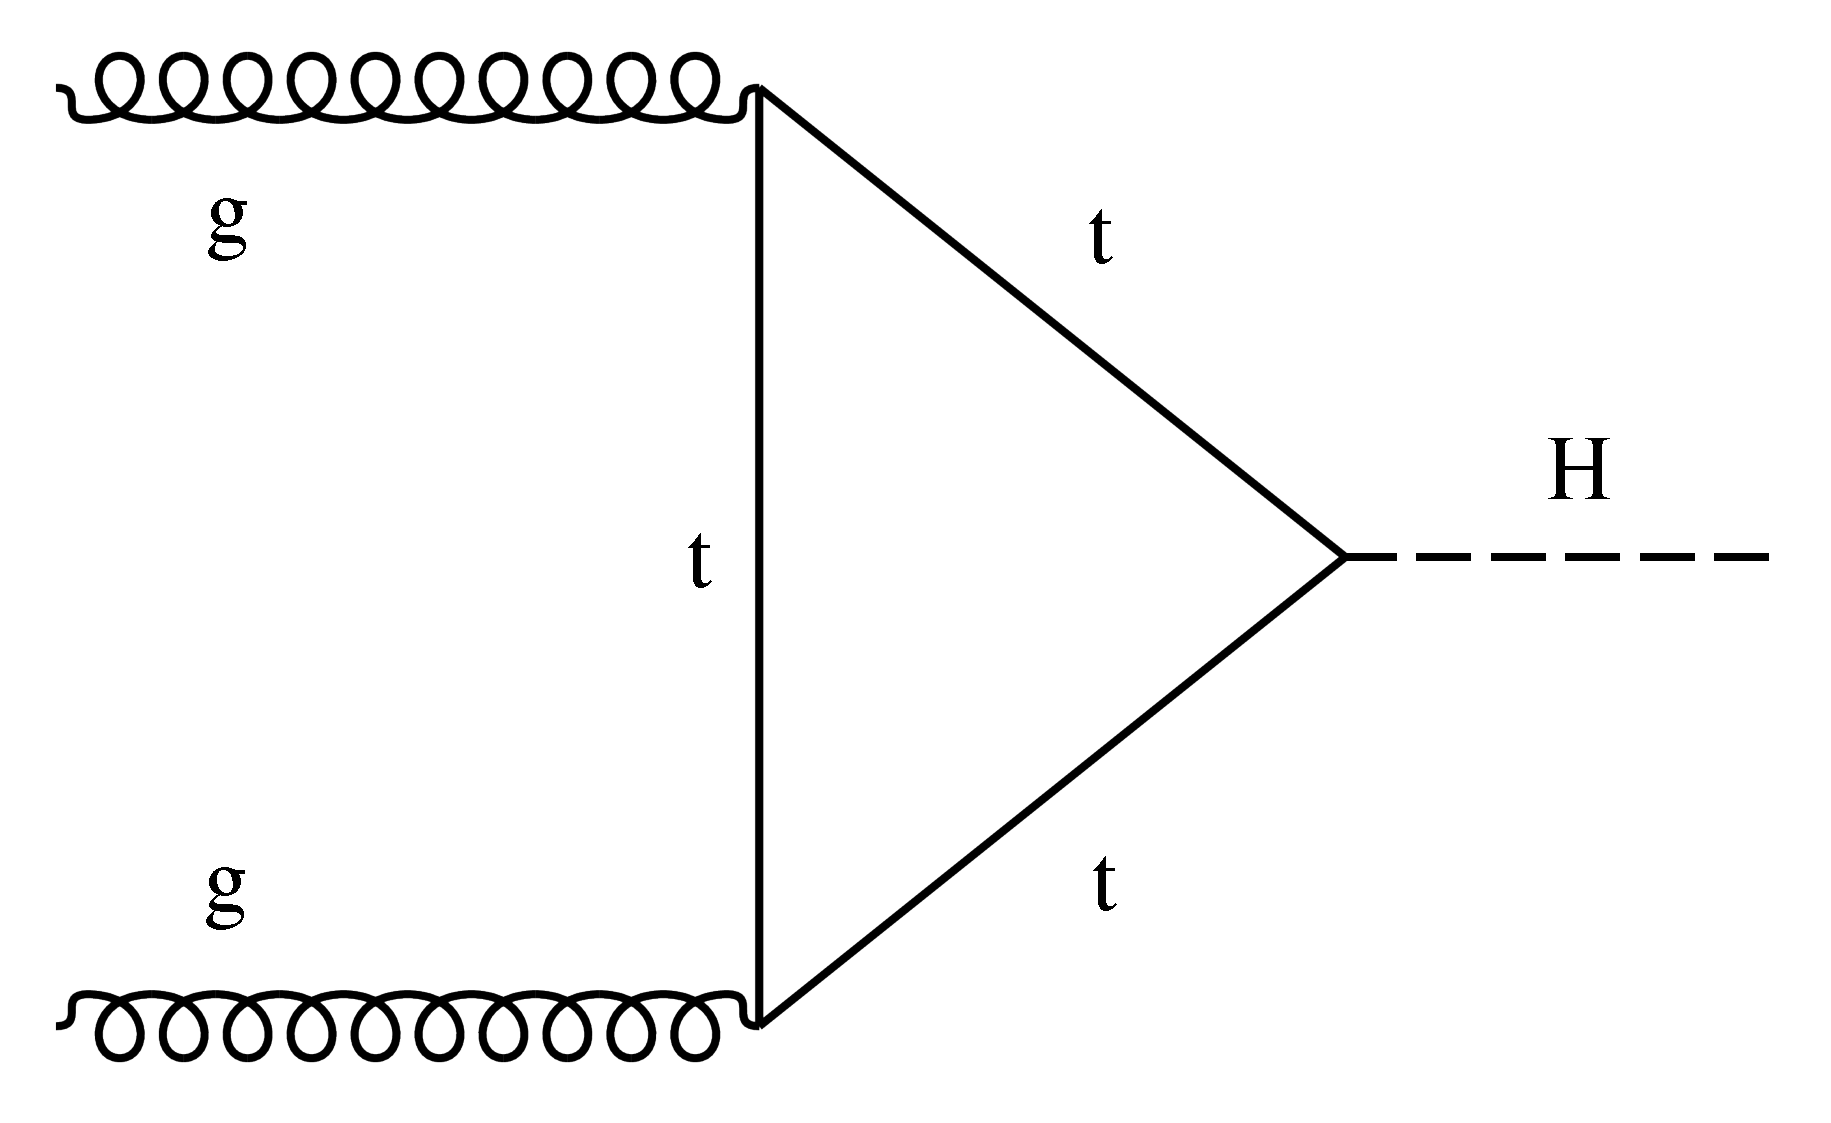
\includegraphics[width=\textwidth]{figures_and_tables/theory/higgs_prod_and_decays/ggf.pdf}
    \caption{Gluon Fusion - ggF}
  \end{subfigure}
  \hfill
  \begin{subfigure}[htbp]{0.48\textwidth}
    \centering
    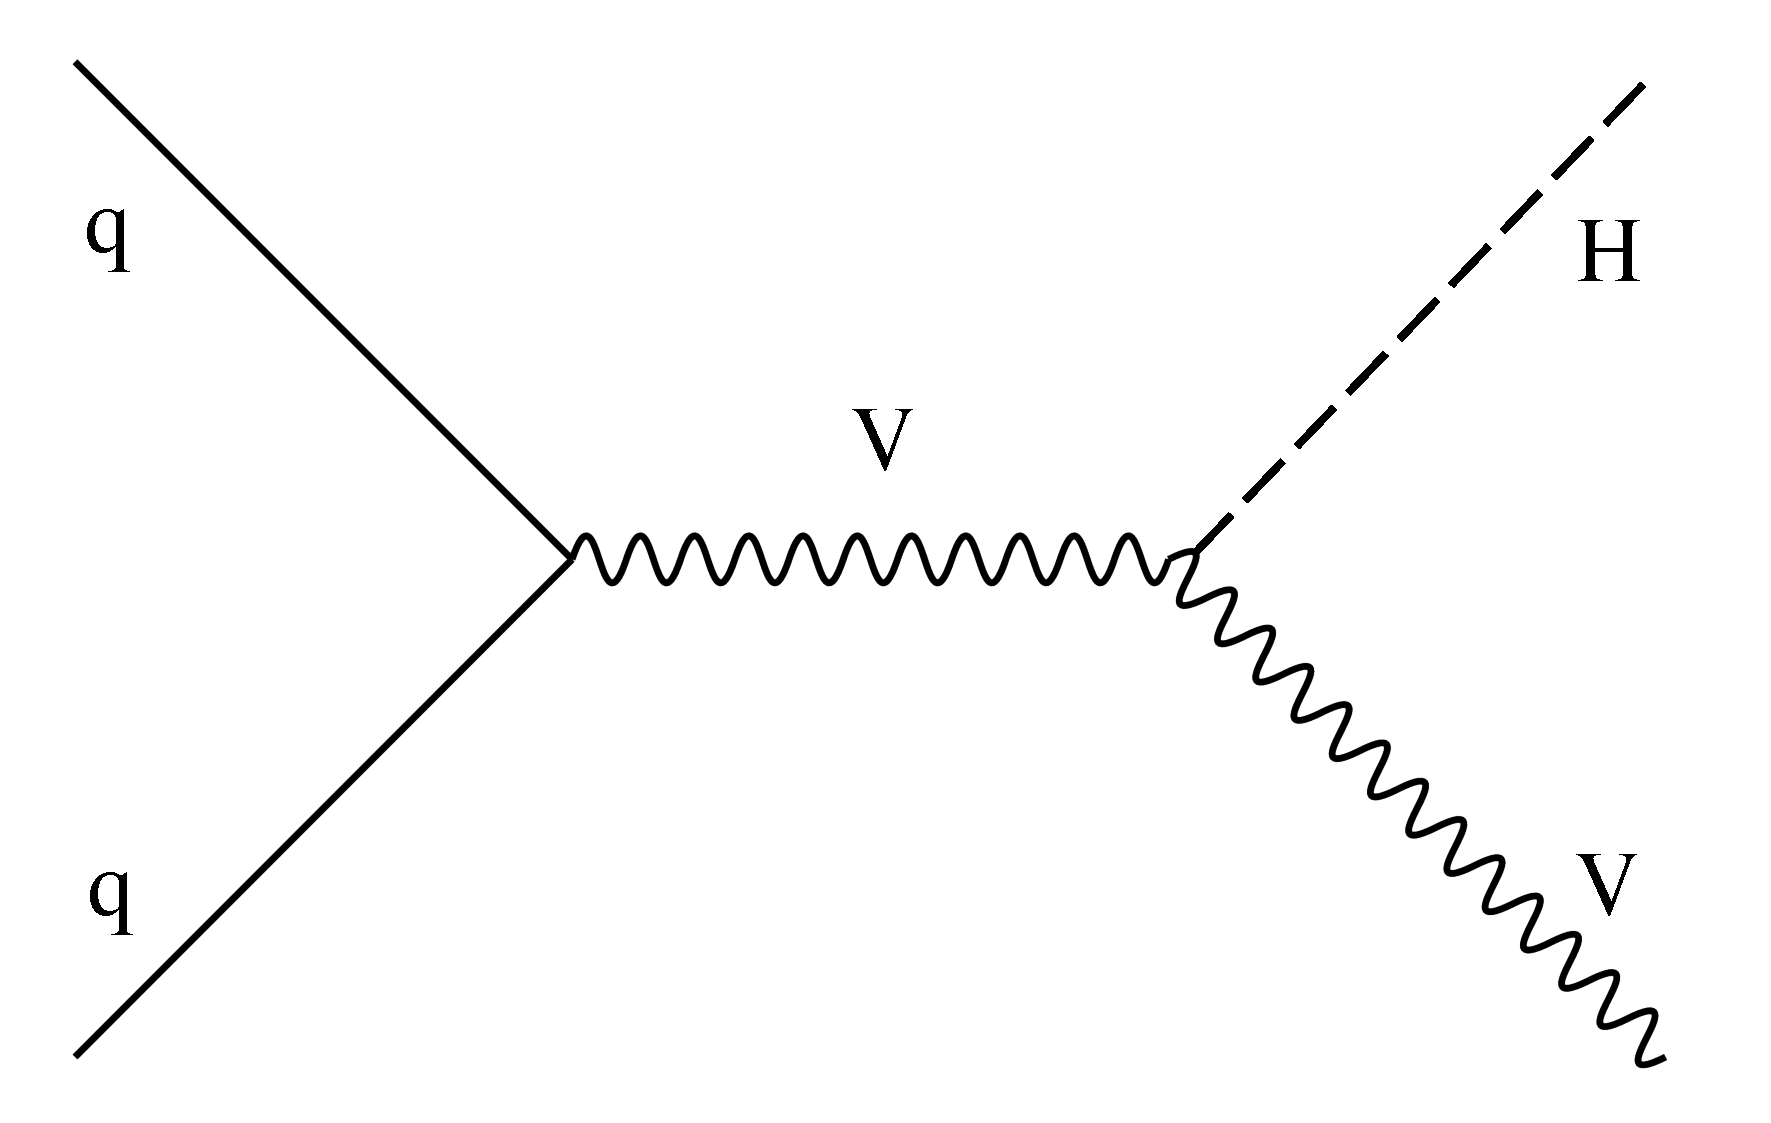
\includegraphics[width=\textwidth]{figures_and_tables/theory/higgs_prod_and_decays/vh.pdf}
    \caption{Associated Vector Boson Production - VH}
  \end{subfigure}
  \begin{subfigure}[htbp]{0.48\textwidth}
    \centering
    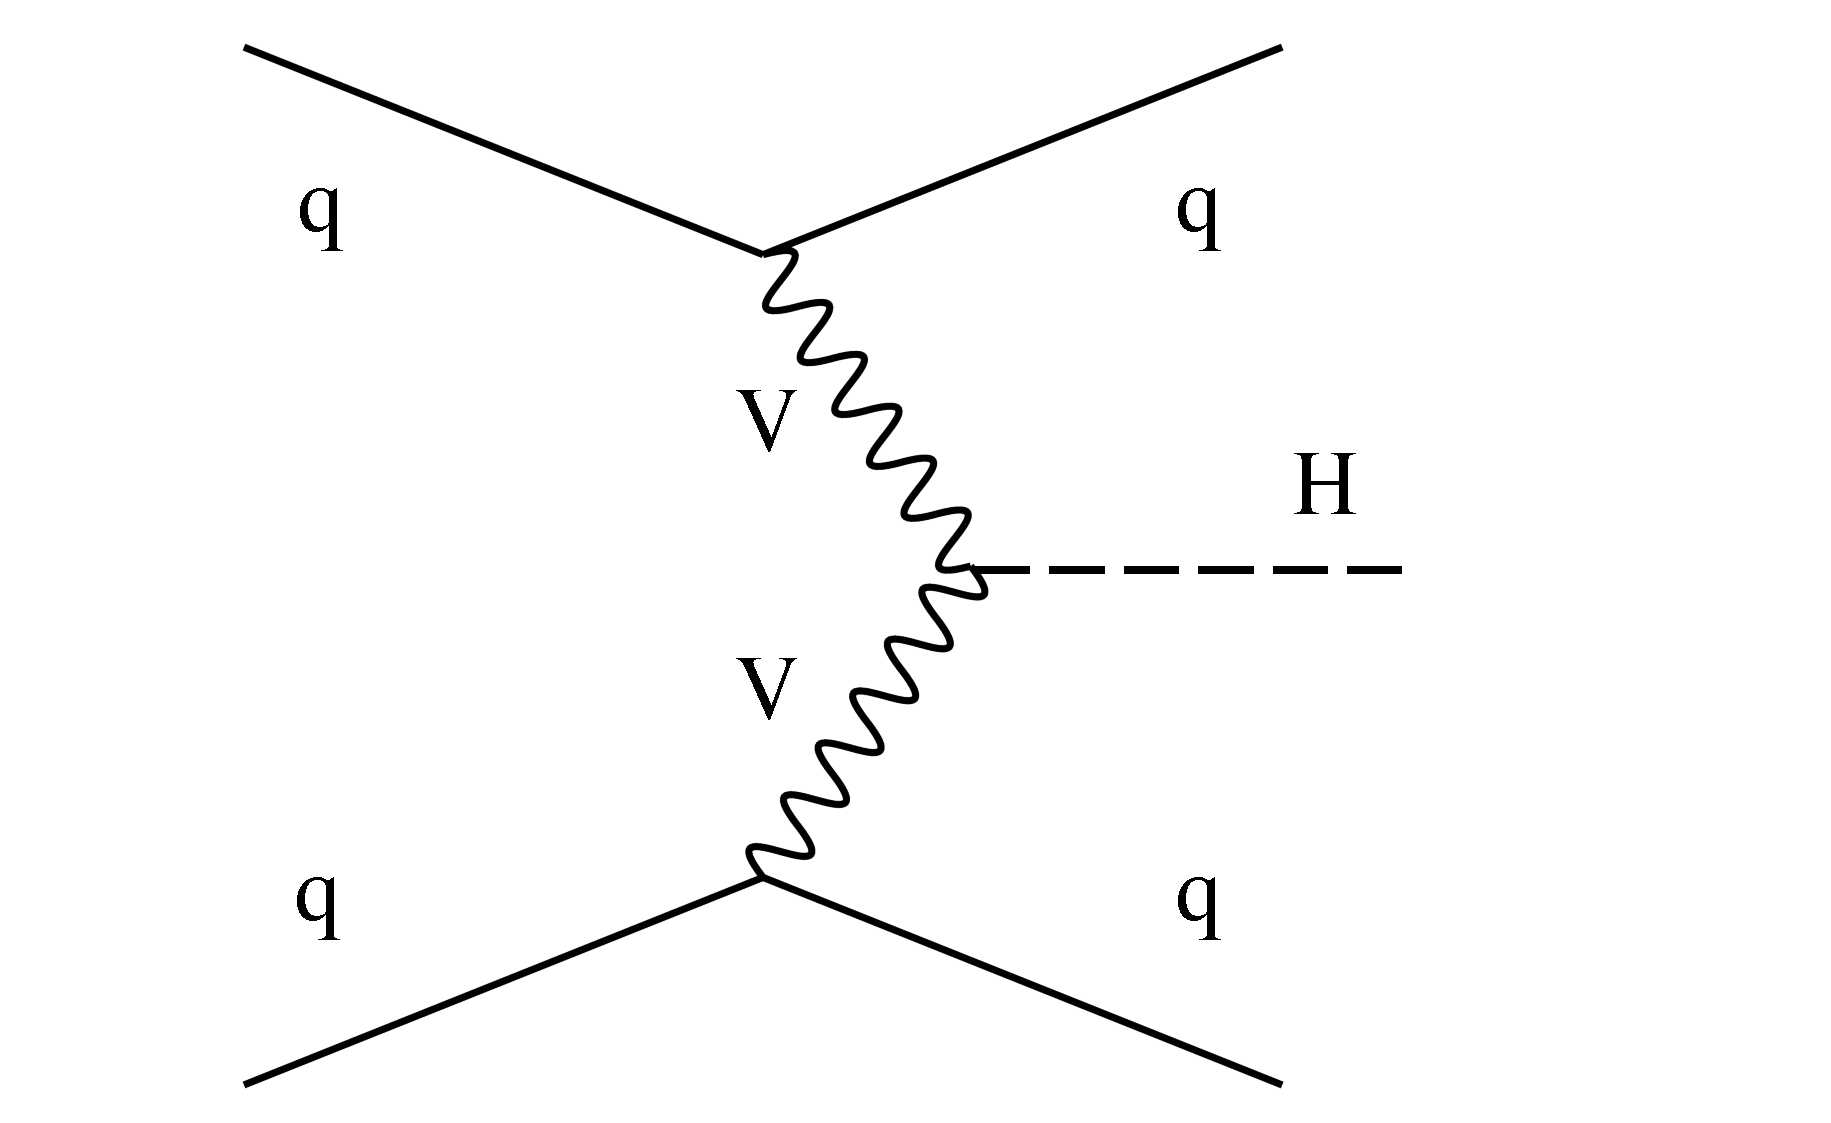
\includegraphics[width=\textwidth]{figures_and_tables/theory/higgs_prod_and_decays/vbf.pdf}
    \caption{Vector Boson Fusion - VBFH}
  \end{subfigure}
  \hfill
  \begin{subfigure}[htbp]{0.48\textwidth}
    \centering
    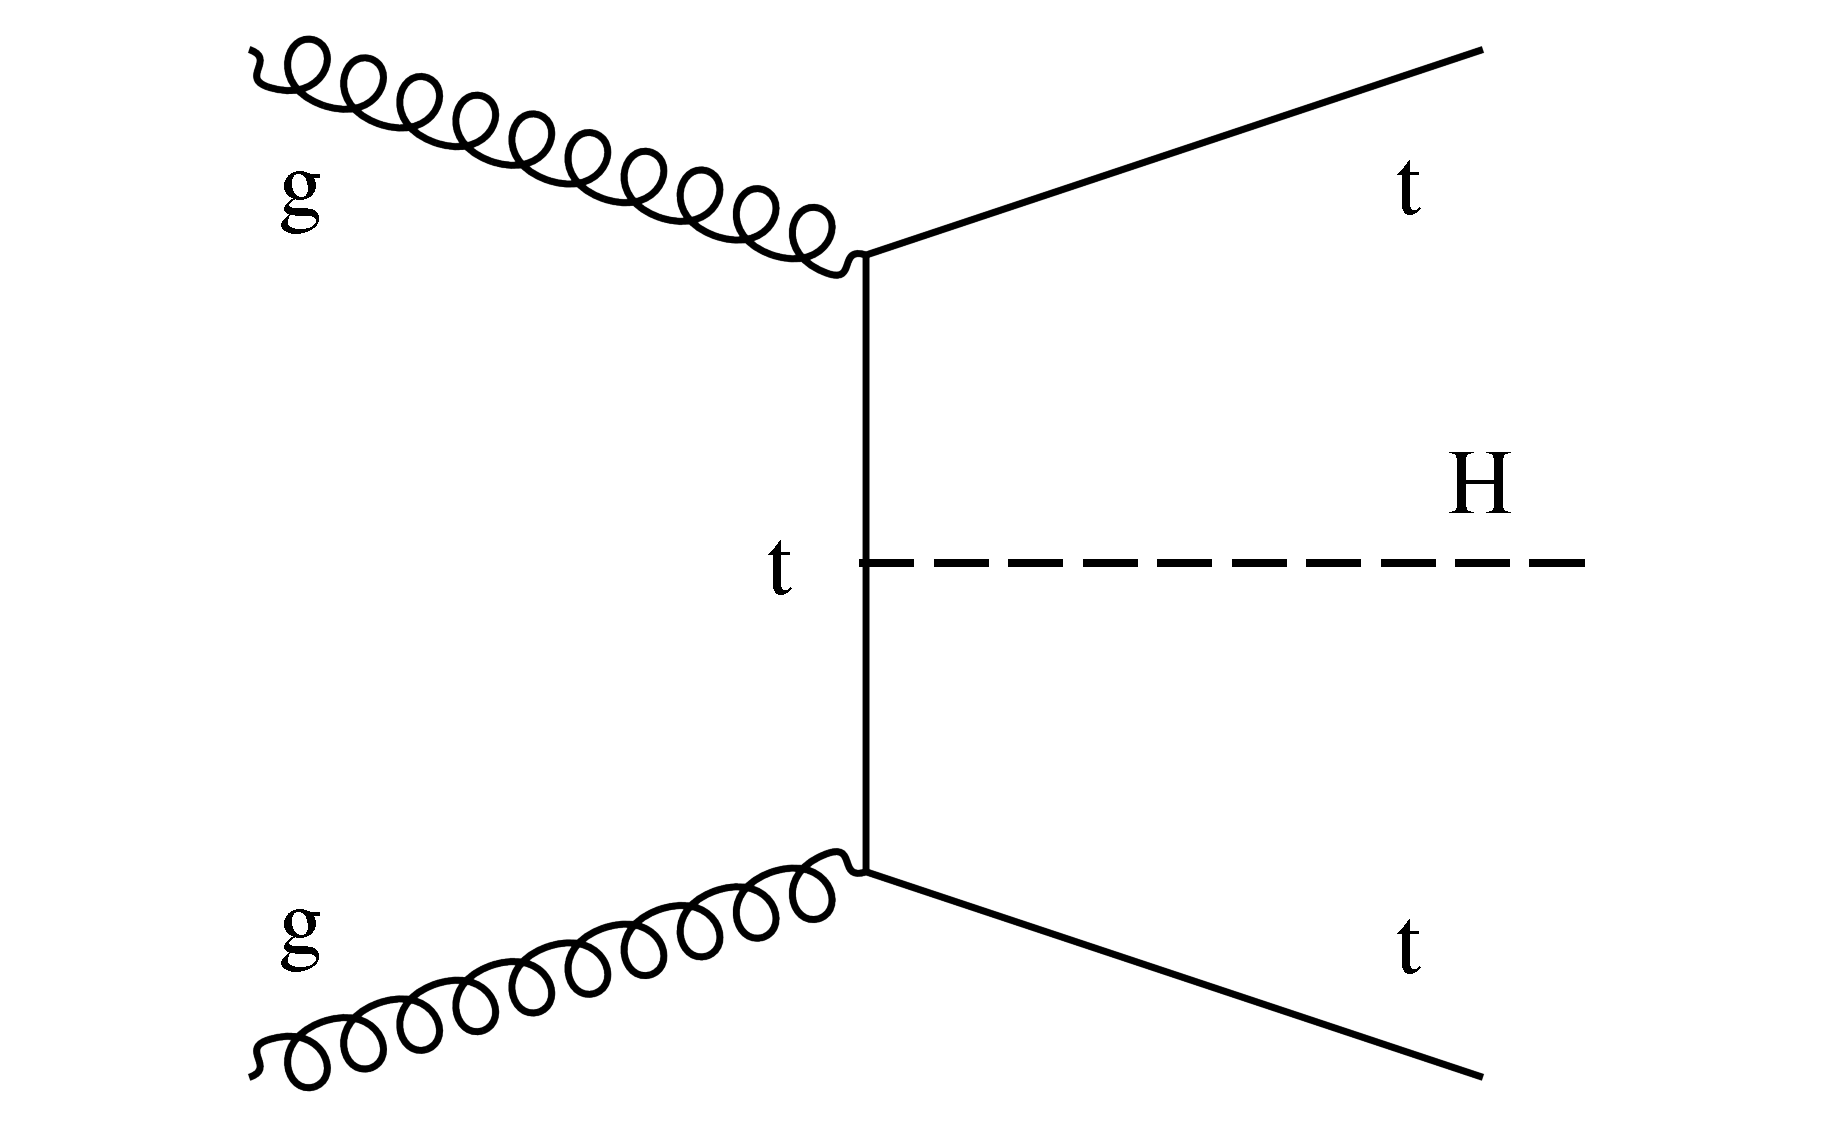
\includegraphics[width=\textwidth]{figures_and_tables/theory/higgs_prod_and_decays/tth.pdf}
    \caption{Associated $t\bar{t}$ Production - ttH}
  \end{subfigure}
  \caption{Example of leading order Standard Model Higgs boson production model diagrams. Source:~\cite{higgs_diagrams}.}
  \label{fig_diagrams_production_modes}
\end{figure}

The Higgs allowed \mbox{\textbf{Decay Channel}}, in the context of the Standard Model, is also a closet set, which have also been subject of study of the "LHC Higgs Cross Section Working Group"~\cite{deFlorian:2016spz}. Figure~\ref{higgs_decays} presents their expected branching ratios.

The largest branching fraction is the decay to a $b\bar{b}$ pair, which is, at $\sqrt{s} = 13$ TeV, more than the double of the next channel. The large cross section does not imply in being the most sensible channel for the Higgs observation. One has to take into account the experimental sensitivity to this final state (which rely on b-tagging techniques) and its enormous QCD background. Tagging on an specific production modes is usually explored in this kind of study~\cite{cms_higgs_to_bbar} to enhance the signal to background ratio. Similar to $b\bar{b}$, decays to other SM dileptons are also usually studied, such as dimuons~\cite{cms_higgs_mumu}, $\tau\tau$~\cite{cms_higgs_to_tautau} and  $c\bar{c}$~\cite{cms_higgs_to_ccbar}. 

Other decays include the $VV$ state, where $V$ is a electroweak vector boson ($Z$~\cite{Sirunyan:2018sgc}, $W^{\pm}$~\cite{Sirunyan:2020tzo} and $\gamma$~\cite{Sirunyan:2020xwk}). Even tough the branching fraction for these ones are relatively smaller, they offer a clear signature for event selection, with reduced QCD background. It is important to notice that $H \rightarrow Z\gamma$ also play a role in this decay mode. CMS (and ATLAS) has a very good sensitivity for leptonic final states of these bosons and for a direct measurement of photons, with resolutions to the order of 1\% for the Higgs. Other channels will have resolutions larger than 10\%~\cite{pdg_2020}.

Gluonic Higgs decays ($H \rightarrow gg$) are allowed in the Standard Model, but they would be overwhelmed by the QCD background. This is considered to be measurable only in the context of a $e^{+}e^{-}$ collider~\cite{Spira:1995rr}.

As already mentioned on Section~\ref{section_sm_higgs_results}, the Higgs was found at CMS and ATLAS in 2012, with Run1 data at $\sqrt{s} =$ 7 and 8 TeV, by investigating the $H \rightarrow ZZ \rightarrow 4l$ and $H \rightarrow \gamma\gamma$ decays. Figures~\ref{higgs_discovery_hgg} and~\ref{higgs_discovery_hzz4l} present the reconstructed final state invariant masses that lead to its discovery. Since then, a broad program have been carried out by both, ATLAS and CMS, to extend the understanding of the Higgs boson to all accessible decays, production modes and also its properties and differential cross section.

% Higgs discovery
\begin{figure}[htbp]
  \centering
  \begin{subfigure}[htbp]{0.48\textwidth}
    \centering
    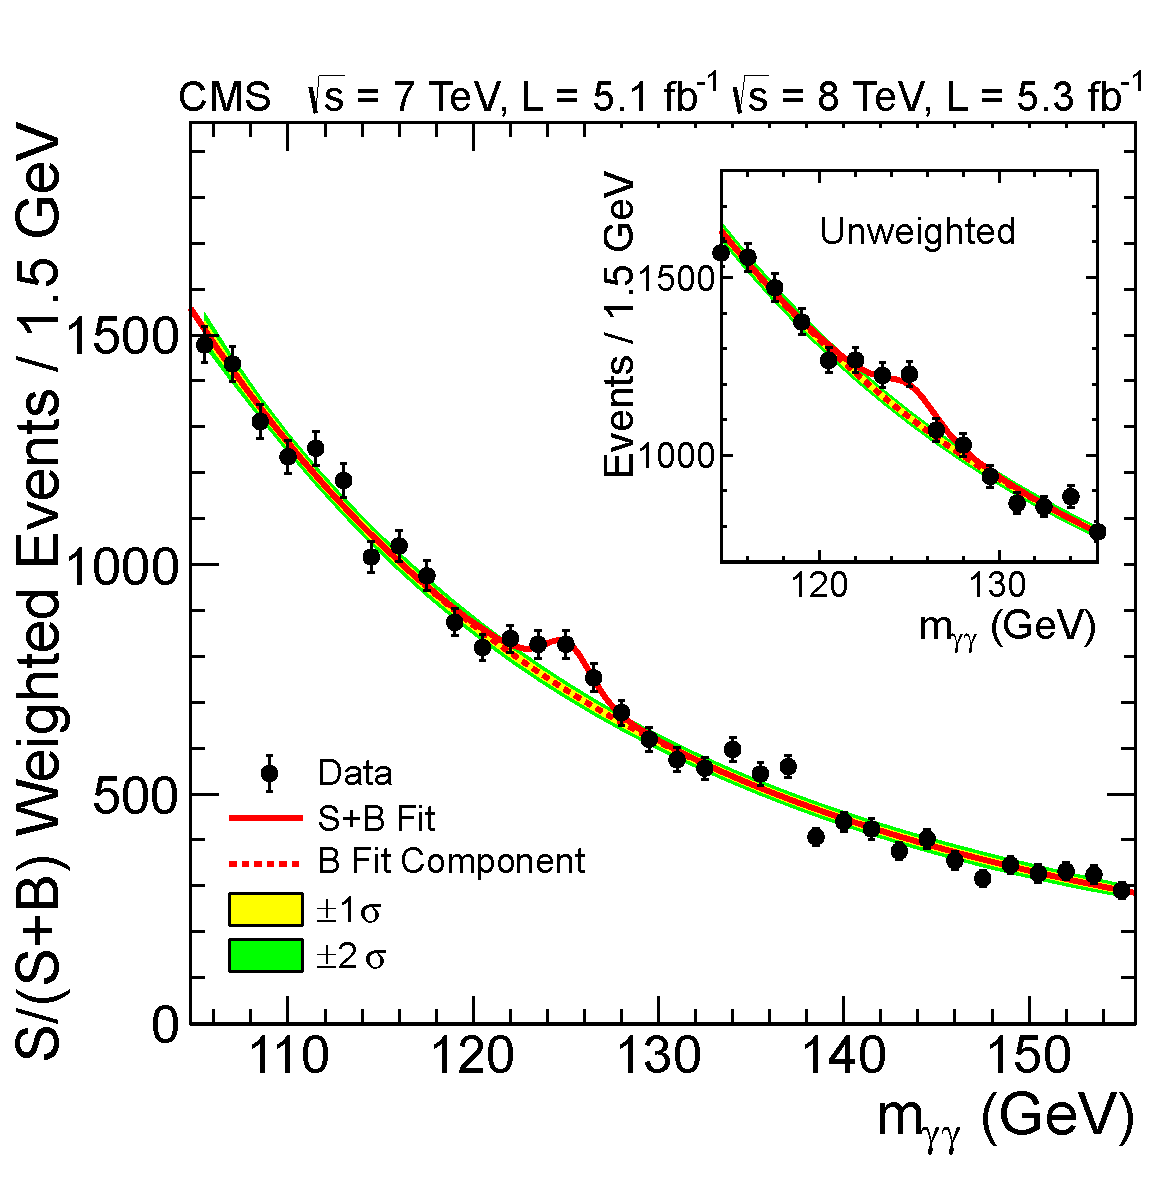
\includegraphics[width=\textwidth]{figures_and_tables/theory/higgs_discovery_hgg.pdf}
    \caption{}
    \label{higgs_discovery_hgg}
  \end{subfigure}
  \hfill
  \begin{subfigure}[htbp]{0.48\textwidth}
    \centering
    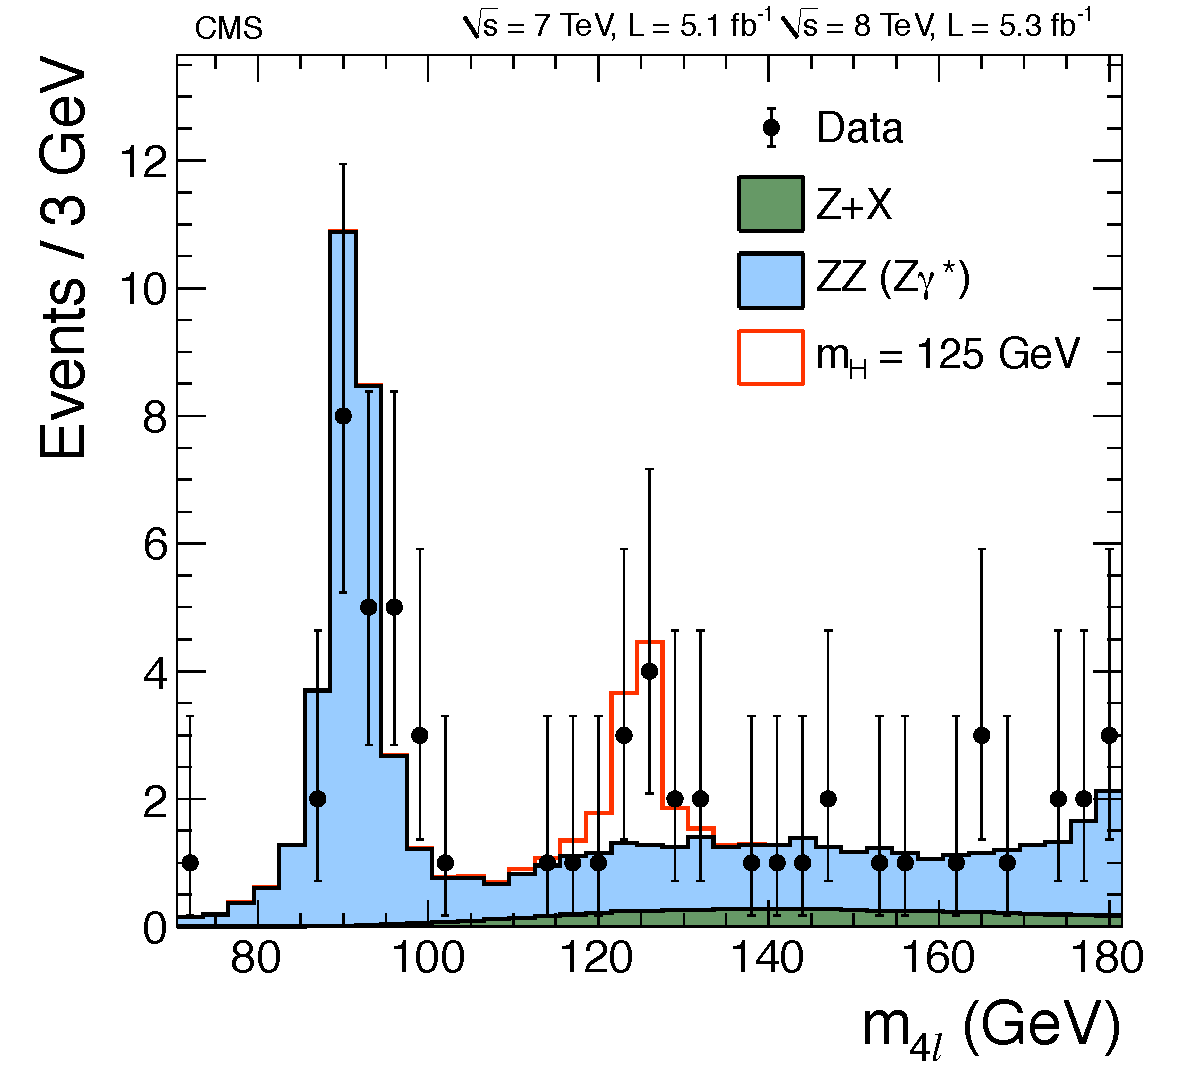
\includegraphics[width=\textwidth]{figures_and_tables/theory/higgs_discovery_hzz4l.pdf}
    \caption{}
    \label{higgs_discovery_hzz4l}
  \end{subfigure}
  \label{higgs_discovery}
  \caption{(a) The diphoton invariant-mass distribution for the 7 and 8 \TeV datasets (points), with each event weighted by the predicted $S/(S+B)$ ratio of its event class. The solid and dotted lines give the results of the signal-plus-background and background-only fit, respectively. The light and dark bands represent the $\pm$1 and $\pm$2 standard deviation uncertainties respectively on the background estimate. The inset shows the corresponding unweighted invariant-mass distribution around \mbox{$m_{\gamma\gamma}$ = 125 \GeV}. Source:~\cite{higgs_discovery_cms}. (b) Distribution of the observed four-lepton invariant mass from the combined 7 and 8 \TeV data 
  for the $\PH \to \cPZ\cPZ\to 4\ell$ analysis (points).
  The prediction for the expected $\cPZ$+X and $\cPZ\cPZ(\cPZ\gamma^*)$ background are shown by the dark and light histogram, respectively. The open histogram gives the expected distribution for a Higgs boson of mass 125 \GeV. Source:~\cite{higgs_discovery_cms}.}
\end{figure}

A complete list of Higgs publications and public result from CMS can be found at~\cite{cms_higgs_publications,cms_higgs_public_results}. With the Higgs measurements being carried out per decay channel, a important effort of combination of these results in performed independently by each collaboration, as well as joint combinations. Some of the Higgs boson measurements by CMS are summarized.

The signal strength modifier is the ratio of the measured cross section or branching ratio over the expected one. 

\begin{equation}
  \mu^{i} = \frac{\sigma^{i}}{\sigma^{i}_{SM}} \qquad\qquad   \mu^{f} = \frac{\mathcal{B}^{i}}{\mathcal{B}^{i}_{SM}}, 
  \label{signal_strength_modifier}
\end{equation}
where $\sigma^{i}$ and $\mathcal{B}^{i}$ stand for the measured cross section and branching ratio of a certain production mode or decay channel, respectively. Figure~\ref{signal_strength_modifier} presents the most updated measurements of $\mu^{i}$ and  $\mu^{f}$ during Run2. The overall combined strength modifier is $\mu=1.02^{+0.07}_{-0.06}$~\cite{cms_higgs_comb_run2}, for $m_{H} = 125.09$ GeV, which shows very good agreement with the SM expectation.

% signal strength modifier - COMB RUn2
\begin{figure}[htbp]
  \centering
  \begin{subfigure}[htbp]{0.48\textwidth}
    \centering
    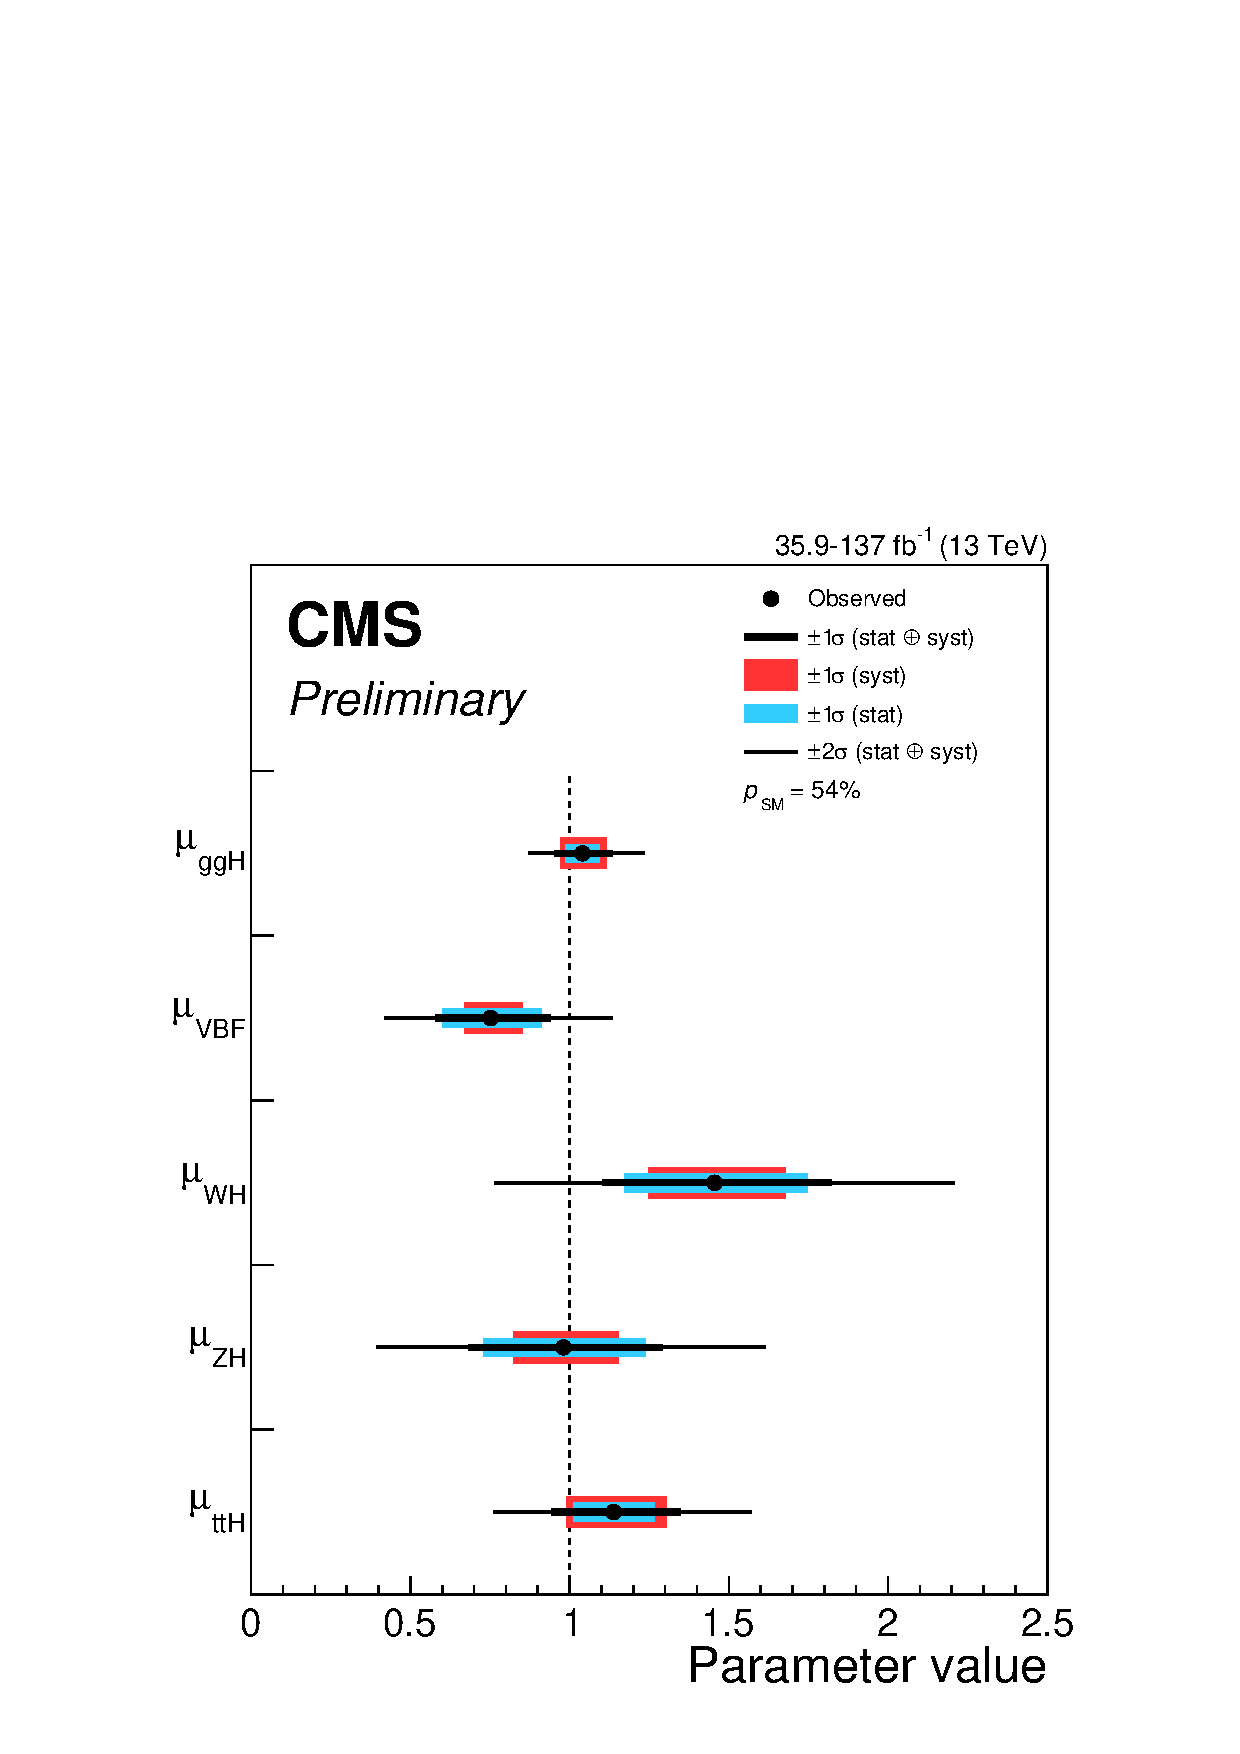
\includegraphics[width=\textwidth]{figures_and_tables/theory/signal_strength_modifier_prod.pdf}
    \caption{ }
    \label{signal_strength_modifier_prod}
  \end{subfigure}
  \hfill
  \begin{subfigure}[htbp]{0.48\textwidth}
    \centering
    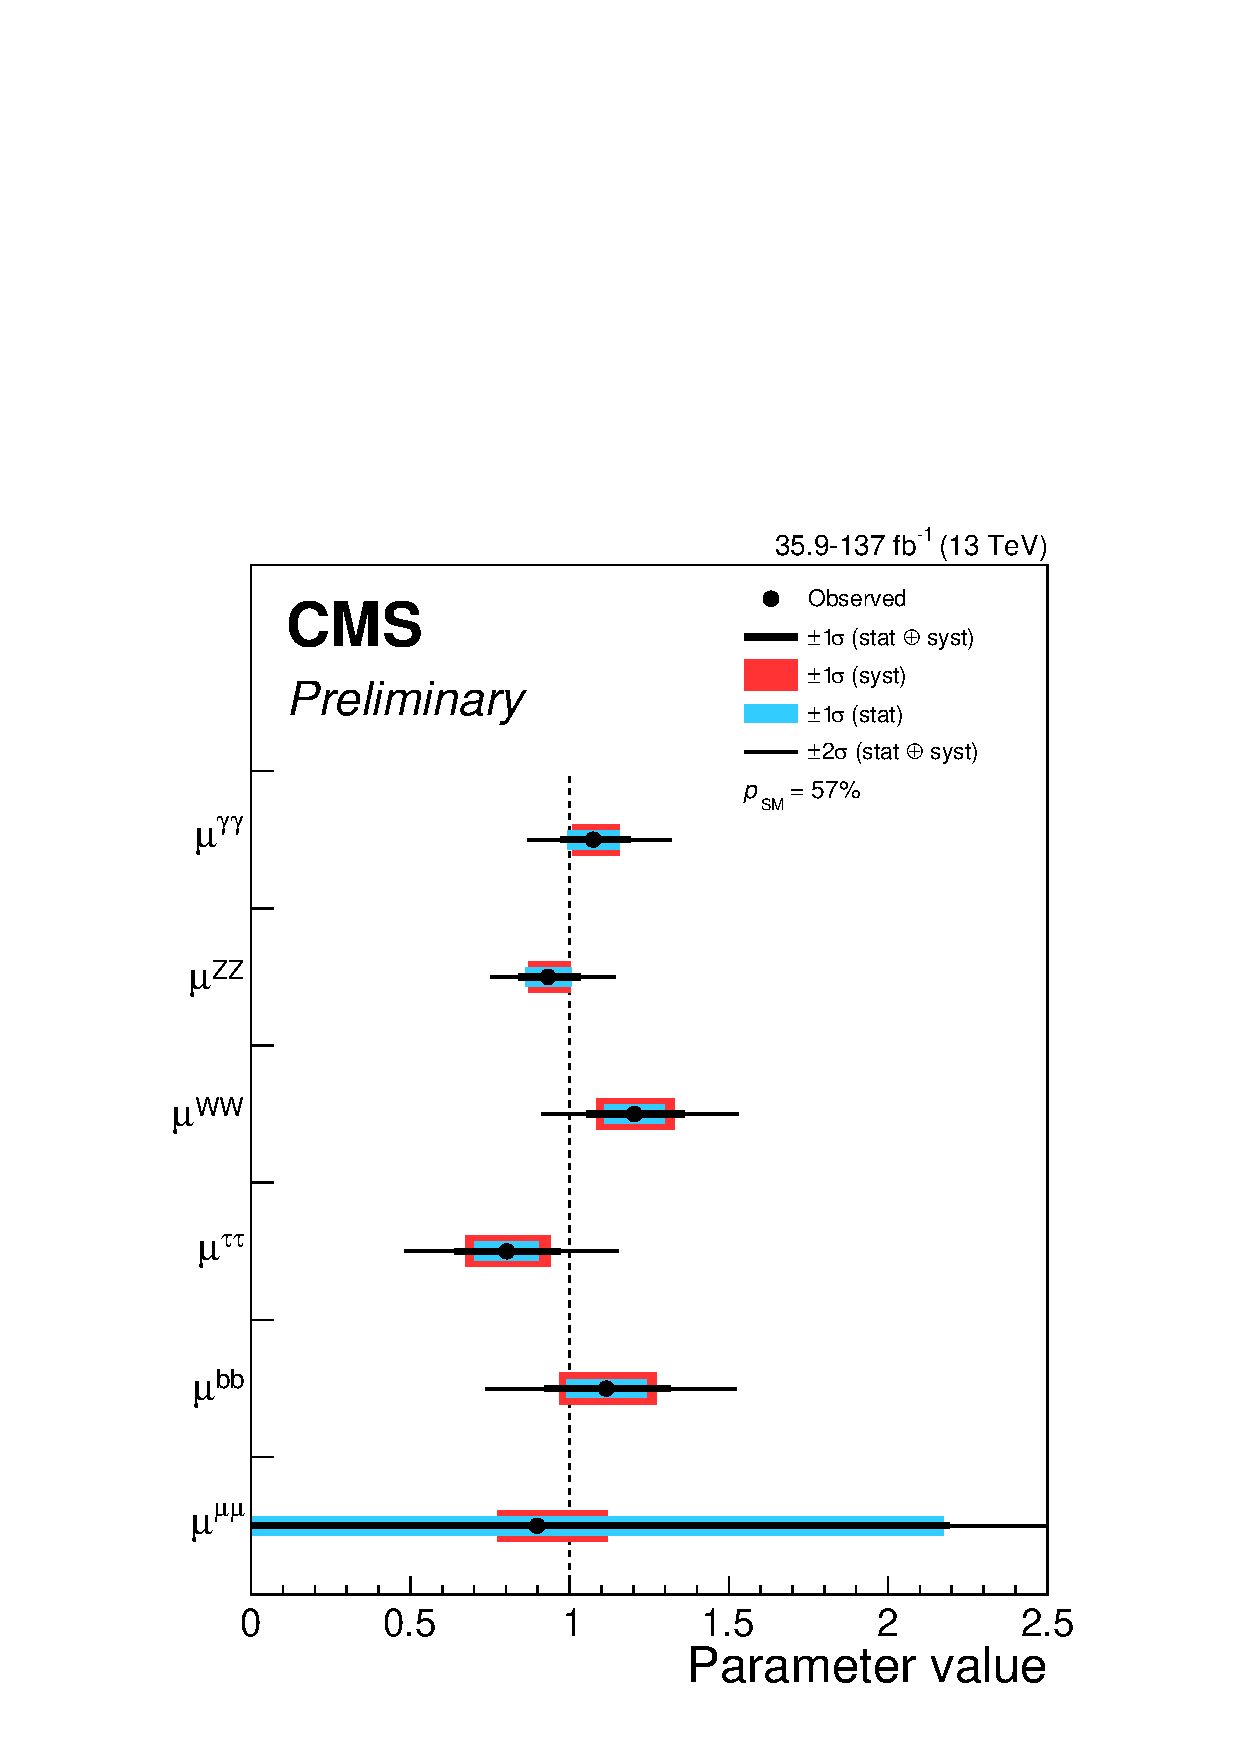
\includegraphics[width=\textwidth]{figures_and_tables/theory/signal_strength_modifier_decay.pdf}
    \caption{ }
    \label{signal_strength_modifier_decay}
  \end{subfigure}
  \caption{Signal strength modifiers for the production modes, (a) $\mu^{i}$, and for the decay channels, (b) $\mu^{f}$. The thick (thin) black lines report the $1\sigma$ ($2\sigma$) confidence intervals. The thick blue and red lines report the statistical and systematic components of the $1\sigma$ confidence intervals. Source:~\cite{cms_higgs_comb_run2}.}
  \label{signal_strength_modifier}
\end{figure}

The Higgs mass was also subject of many study, here we quote the results on Figure~\ref{higgs_mass}~\cite{Sirunyan:2020xwk}, for Run1 and partial Run2 datasets, for both $H \rightarrow ZZ \rightarrow 4l$ and $H \rightarrow \gamma\gamma$ decays. The combined measurement is $m_H = 125.38 \pm 0.14$ GeV. This is the \textit{state-of-art} value for the Higgs mass.

% Higgs mass
\begin{figure}[htbp]
  \centering
  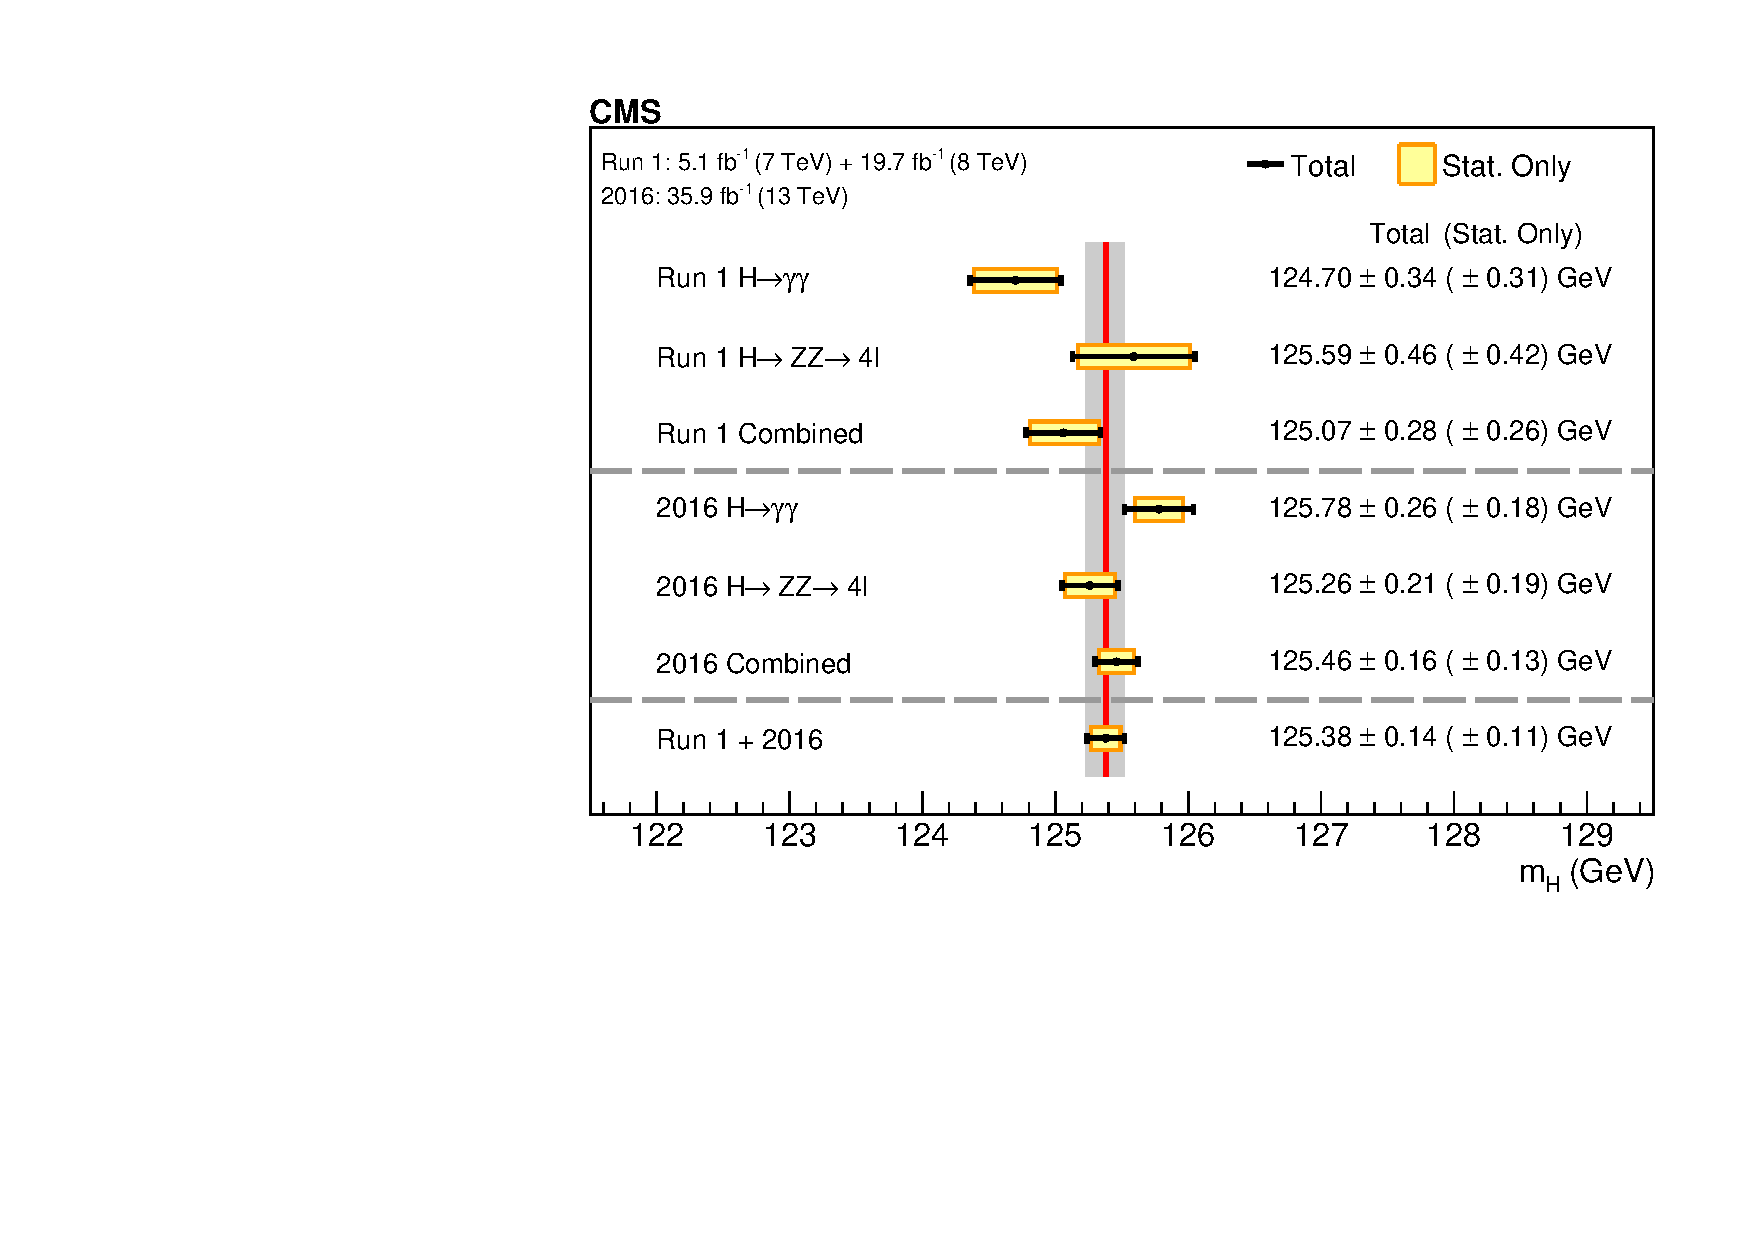
\includegraphics[width=0.7\textwidth]{figures_and_tables/theory/cms_higgs_mass.pdf}
  \caption{A summary of the measured Higgs boson mass in the $H \rightarrow ZZ \rightarrow 4l$ and $H \rightarrow \gamma\gamma$ decay channels, and for the combination of the two is presented here. The statistical (wider, yellow-shaded bands), and total (black error bars) uncertainties are indicated. The (red) vertical line and corresponding (grey) shaded column indicate the central value and the total uncertainty of the Run 1 + 2016 combined measurement, respectively. Source:~\cite{Sirunyan:2020xwk}.}
  \label{higgs_mass}
\end{figure}

Other properties studied comprehends its quantum numbers. The Landau-Yang theorem~\cite{Landau:1948kw,Yang:1950rg} rules out the spin-1 possibility, based on its observation on the $\gamma\gamma$ channel. All the tests conducted, so far, support the $J^P = 0^+$ hypothesis~\cite{cms_higgs_spin_tests}.

A recent very relevant Higgs result published by CMS is the evidence of the $H \rightarrow \mu\mu$ decay~\cite{cms_higgs_mumu}. In this paper it is reported an excess on data, with respect to the background only hypothesis, with 3$\sigma$ of significance. This is the first evidence of the Higgs coupling to second generation fermions. Figure~\ref{h_to_mumu_result} presents a weighted invariant mass distribution of the dimuon system ($m_{\mu\mu}$) for all the categories included in this analysis.

% H to mumu
\begin{figure}[htbp]
  \centering
  \begin{subfigure}[htbp]{0.48\textwidth}
    \centering
    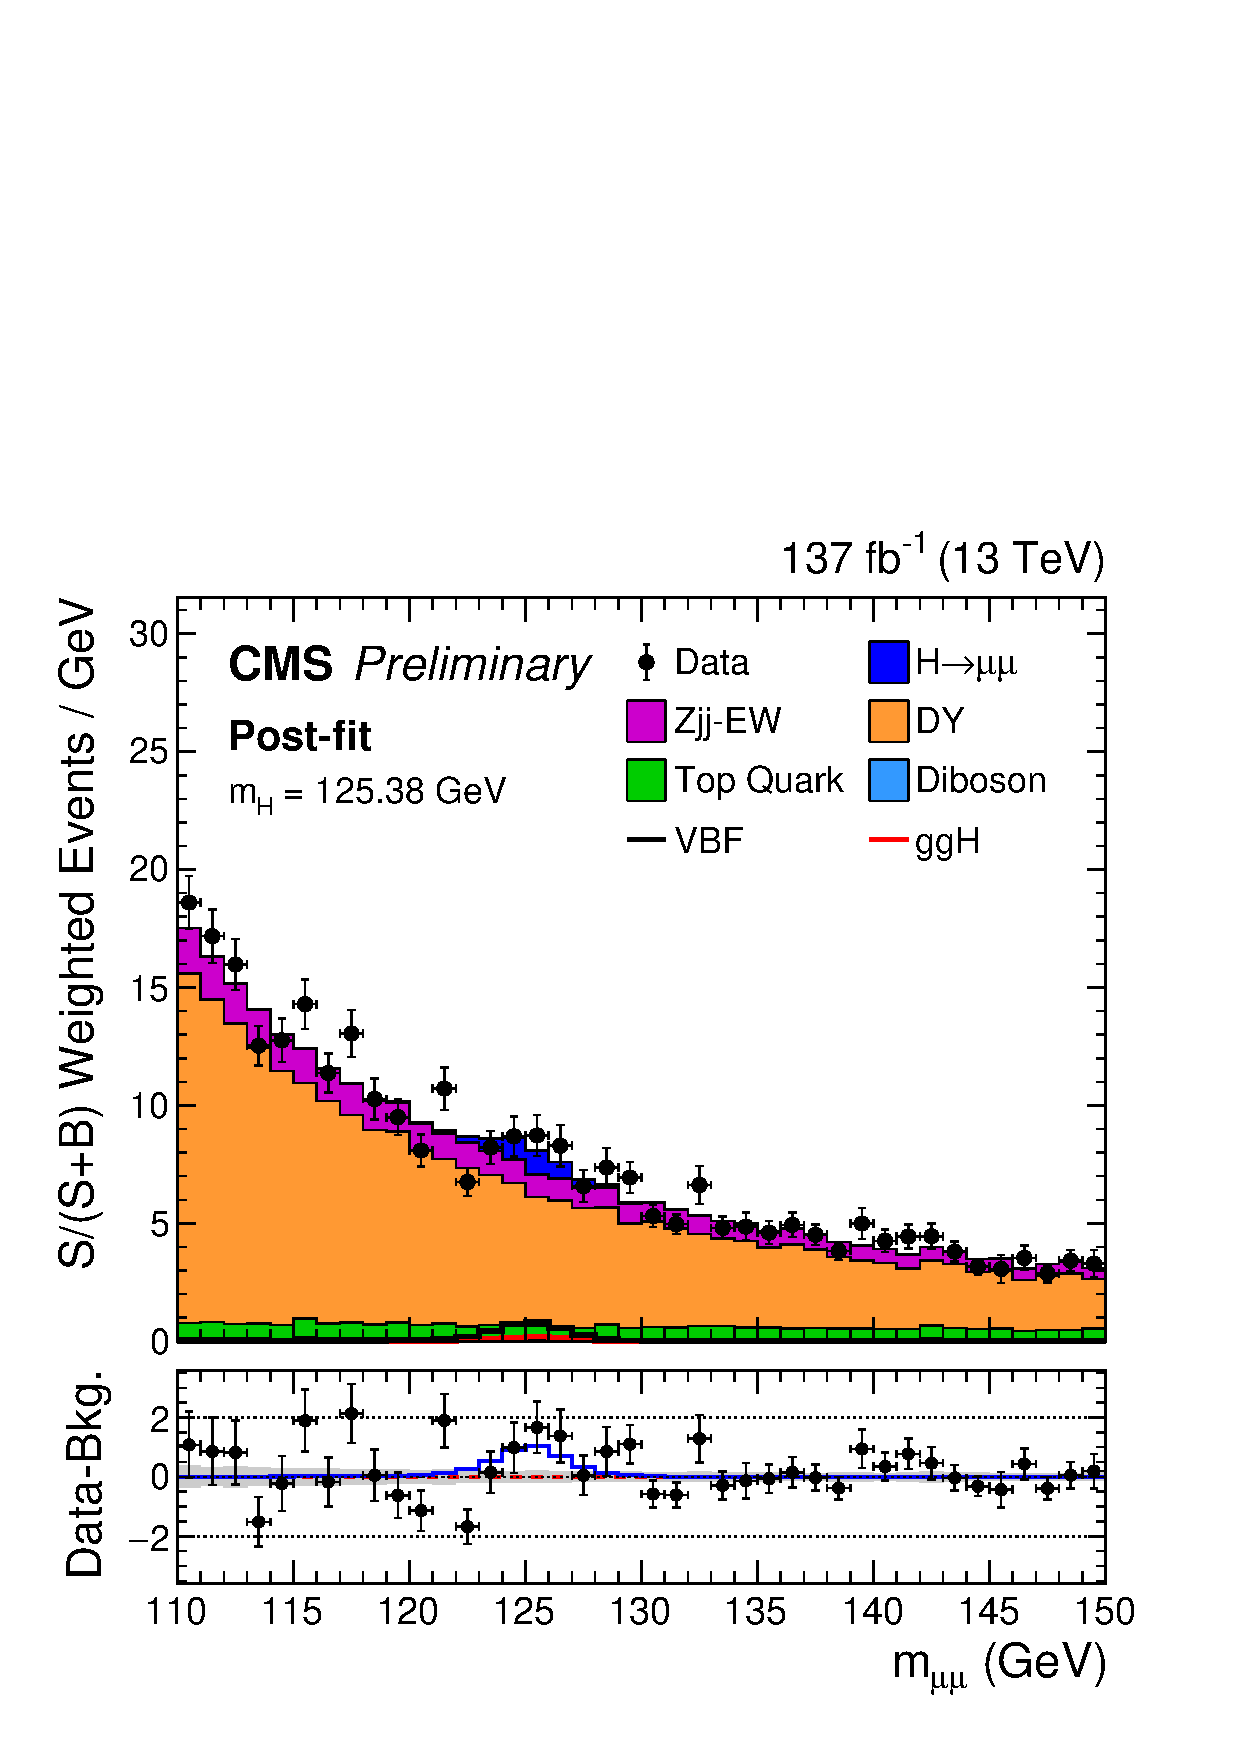
\includegraphics[width=\textwidth]{figures_and_tables/theory/h_to_mumu_result.pdf}
    \caption{}
    \label{h_to_mumu_result}
  \end{subfigure}
  \hfill
  \begin{subfigure}[htbp]{0.48\textwidth}
    \centering
    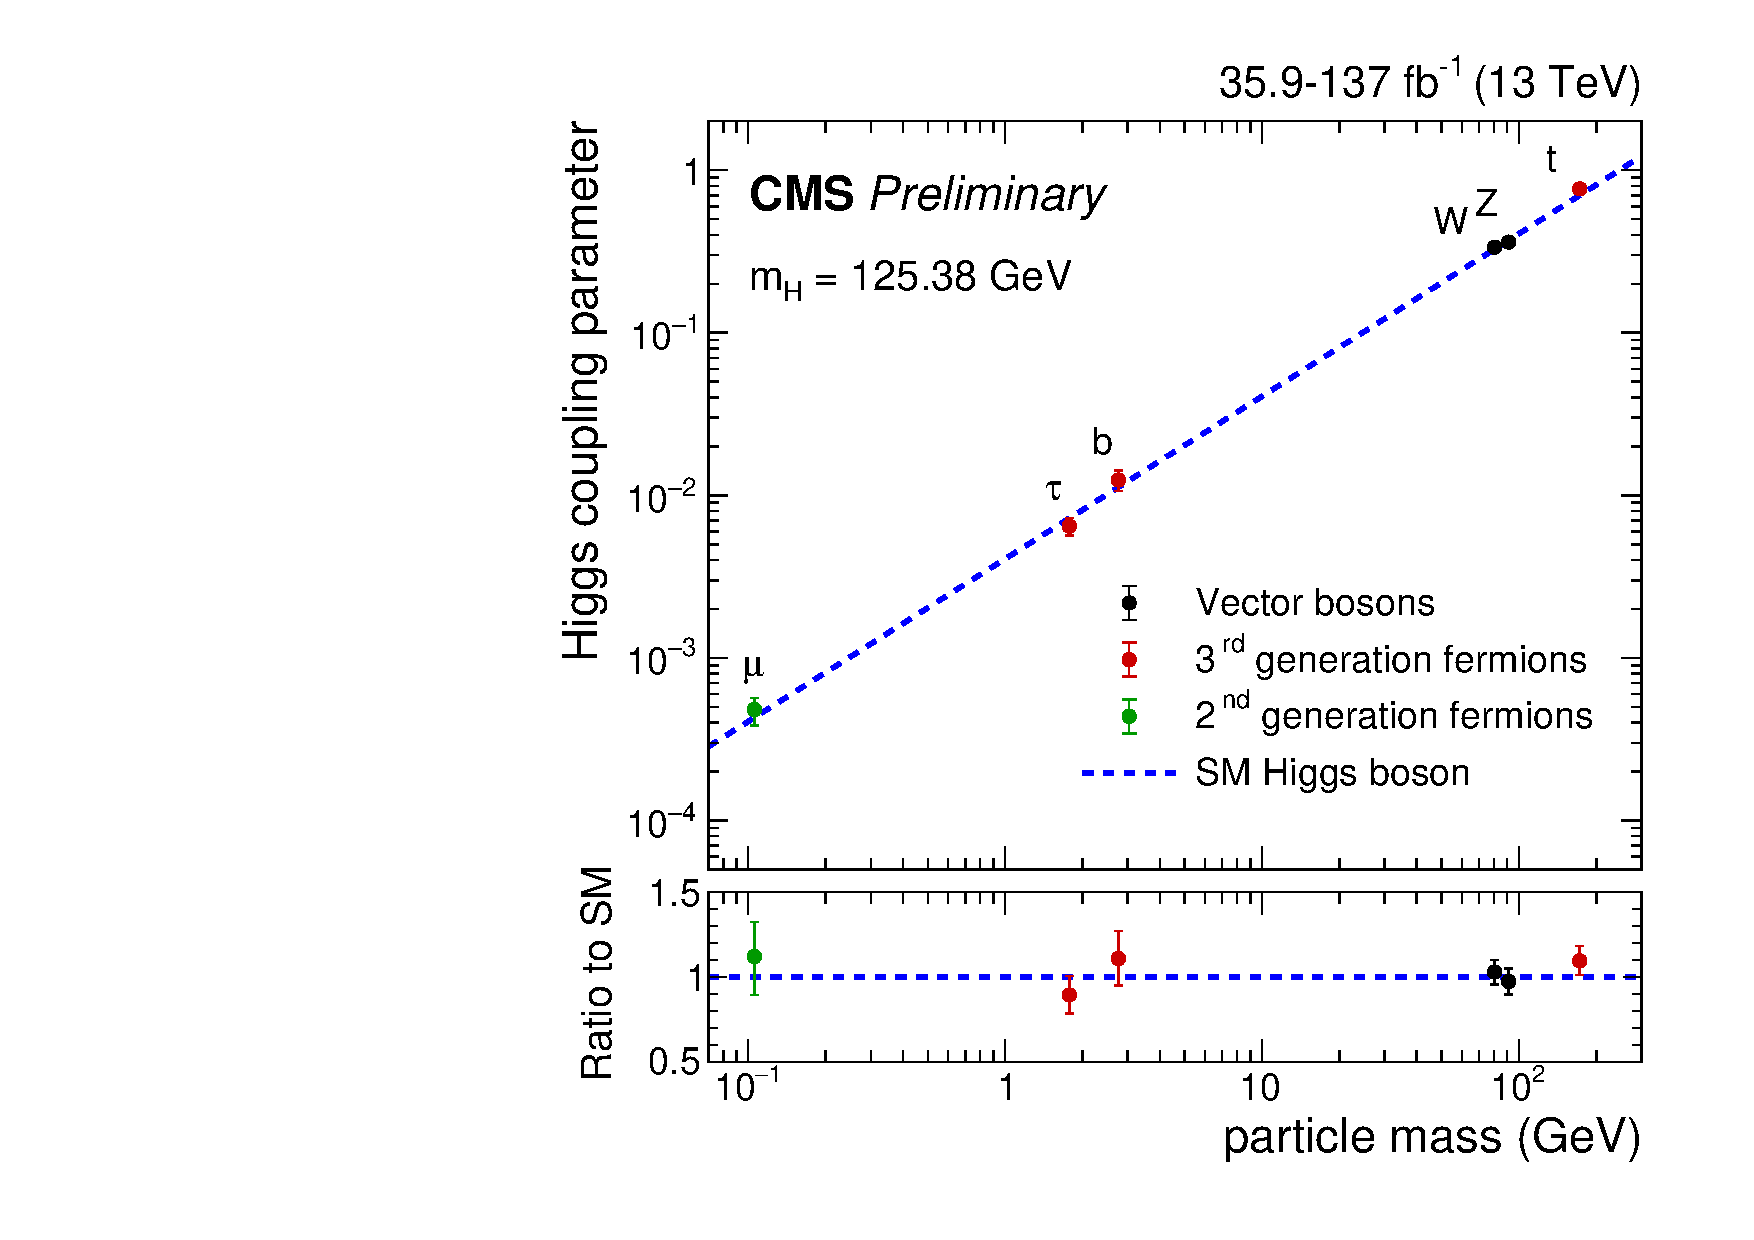
\includegraphics[width=\textwidth]{figures_and_tables/theory/higgs_coups.pdf}
    \caption{}
    \label{higgs_coups}
  \end{subfigure}
  \label{h_to_mumu_result_higgs_coups}
  \caption{(a) T the $m_{\mu\mu}$ distribution for the weighted combination of all event categories used in the analysis. The upper panel is dominated by the gluon-gluon fusion categories with many data events but relatively small $S/(S + B)$. The lower panel shows the residuals after background subtraction, with the best-fit SM $H \rightarrow \mu\mu$ signal contribution with $m_H = 125.38$ GeV indicated by the red line. The measured signal strength is ${1.19^{+0.41}_{-0.39}(\mathrm{stat})^{+0.17}_{-0.16}(\mathrm{sys})}$. Source:~\cite{cms_higgs_mumu}. (b) The best-fit estimates for the reduced coupling modifiers extracted for fermions and weak bosons from the resolved $\kappa$-framework model compared to their corresponding prediction from the SM. The error bars represent 68\% CL intervals for the measured parameters. The lower panel shows the ratios of the measured coupling modifiers values to their SM predictions. Source:~\cite{cms_higgs_mumu}.}
\end{figure}

The same note also updates the coupling constant modifier by combining the new results for $H \rightarrow \mu\mu$ with previous Higgs results from Run2~\cite{cms_higgs_comb_run2}. The measured parameters are presented at Figure~\ref{higgs_coups} and they also present very good agreement with the SM prediction, where the coupling constants to fermions is proportional to the fermion mass($M_{f}$), while for electroweak boson, it is proportional to the square of the boson mass ($M_{V}$). The fit results are scaled to the reduced coupling strength modifiers, defined as $y_V=\sqrt{\kappa_V}\frac{m_V}{\nu}$ and $y_f=\kappa_f\frac{m_F}{\nu}$, where $\nu$ is the vacuum expectation value of the Higgs field of 246.22 GeV.
